% Options for packages loaded elsewhere
\PassOptionsToPackage{unicode}{hyperref}
\PassOptionsToPackage{hyphens}{url}
%
\documentclass[
]{article}
\usepackage{amsmath,amssymb}
\usepackage{iftex}
\ifPDFTeX
  \usepackage[T1]{fontenc}
  \usepackage[utf8]{inputenc}
  \usepackage{textcomp} % provide euro and other symbols
\else % if luatex or xetex
  \usepackage{unicode-math} % this also loads fontspec
  \defaultfontfeatures{Scale=MatchLowercase}
  \defaultfontfeatures[\rmfamily]{Ligatures=TeX,Scale=1}
\fi
\usepackage{lmodern}
\ifPDFTeX\else
  % xetex/luatex font selection
\fi
% Use upquote if available, for straight quotes in verbatim environments
\IfFileExists{upquote.sty}{\usepackage{upquote}}{}
\IfFileExists{microtype.sty}{% use microtype if available
  \usepackage[]{microtype}
  \UseMicrotypeSet[protrusion]{basicmath} % disable protrusion for tt fonts
}{}
\makeatletter
\@ifundefined{KOMAClassName}{% if non-KOMA class
  \IfFileExists{parskip.sty}{%
    \usepackage{parskip}
  }{% else
    \setlength{\parindent}{0pt}
    \setlength{\parskip}{6pt plus 2pt minus 1pt}}
}{% if KOMA class
  \KOMAoptions{parskip=half}}
\makeatother
\usepackage{xcolor}
\usepackage[margin=1in]{geometry}
\usepackage{longtable,booktabs,array}
\usepackage{calc} % for calculating minipage widths
% Correct order of tables after \paragraph or \subparagraph
\usepackage{etoolbox}
\makeatletter
\patchcmd\longtable{\par}{\if@noskipsec\mbox{}\fi\par}{}{}
\makeatother
% Allow footnotes in longtable head/foot
\IfFileExists{footnotehyper.sty}{\usepackage{footnotehyper}}{\usepackage{footnote}}
\makesavenoteenv{longtable}
\usepackage{graphicx}
\makeatletter
\def\maxwidth{\ifdim\Gin@nat@width>\linewidth\linewidth\else\Gin@nat@width\fi}
\def\maxheight{\ifdim\Gin@nat@height>\textheight\textheight\else\Gin@nat@height\fi}
\makeatother
% Scale images if necessary, so that they will not overflow the page
% margins by default, and it is still possible to overwrite the defaults
% using explicit options in \includegraphics[width, height, ...]{}
\setkeys{Gin}{width=\maxwidth,height=\maxheight,keepaspectratio}
% Set default figure placement to htbp
\makeatletter
\def\fps@figure{htbp}
\makeatother
\setlength{\emergencystretch}{3em} % prevent overfull lines
\providecommand{\tightlist}{%
  \setlength{\itemsep}{0pt}\setlength{\parskip}{0pt}}
\setcounter{secnumdepth}{5}
\newlength{\cslhangindent}
\setlength{\cslhangindent}{1.5em}
\newlength{\csllabelwidth}
\setlength{\csllabelwidth}{3em}
\newlength{\cslentryspacingunit} % times entry-spacing
\setlength{\cslentryspacingunit}{\parskip}
\newenvironment{CSLReferences}[2] % #1 hanging-ident, #2 entry spacing
 {% don't indent paragraphs
  \setlength{\parindent}{0pt}
  % turn on hanging indent if param 1 is 1
  \ifodd #1
  \let\oldpar\par
  \def\par{\hangindent=\cslhangindent\oldpar}
  \fi
  % set entry spacing
  \setlength{\parskip}{#2\cslentryspacingunit}
 }%
 {}
\usepackage{calc}
\newcommand{\CSLBlock}[1]{#1\hfill\break}
\newcommand{\CSLLeftMargin}[1]{\parbox[t]{\csllabelwidth}{#1}}
\newcommand{\CSLRightInline}[1]{\parbox[t]{\linewidth - \csllabelwidth}{#1}\break}
\newcommand{\CSLIndent}[1]{\hspace{\cslhangindent}#1}
\usepackage{float} \floatplacement{figure}{H} \newcommand{\beginsupplement}{\setcounter{table}{0}  \renewcommand{\thetable}{A\arabic{table}} \setcounter{figure}{0} \renewcommand{\thefigure}{A\arabic{figure}}}
\ifLuaTeX
  \usepackage{selnolig}  % disable illegal ligatures
\fi
\IfFileExists{bookmark.sty}{\usepackage{bookmark}}{\usepackage{hyperref}}
\IfFileExists{xurl.sty}{\usepackage{xurl}}{} % add URL line breaks if available
\urlstyle{same}
\hypersetup{
  pdftitle={Binocular integration of chromatic and luminance signals},
  hidelinks,
  pdfcreator={LaTeX via pandoc}}

\title{Binocular integration of chromatic and luminance signals}
\author{Daniel H. Baker, Kirralise J. Hansford, Federico G. Segala, Annie Y. Morsi,\\
Rowan J. Huxley, Joel T. Martin, Maya Rockman \& Alex R. Wade}
\date{2024-03-09}

\begin{document}
\maketitle

\hypertarget{abstract}{%
\section{Abstract}\label{abstract}}

\hypertarget{introduction}{%
\section{Introduction}\label{introduction}}

The process by which the brain combines independent inputs is of fundamental importance for understanding sensory perception. Binocular vision is a useful test-case for determining the general principles involved in neural signal combination, as our brains combine the inputs from the left and right eyes to provide binocular single vision. In recent years our understanding has been facilitated by the development of binocular gain control models that provide a framework to interpret empirical data across multiple techniques, including psychophysics (Meese et al., 2006), EEG (Baker \& Wade, 2017), fMRI (Moradi \& Heeger, 2009) and pupillometry (Segala et al., 2023). However, the majority of this work has used achromatic (black and white) stimuli; we know comparatively little about how chromatic signals are combined binocularly, or about how signals in different ocular and chromatic channels interact. In this study we use psychophysical detection and discrimination paradigms to explore binocular interactions in the chromatic pathways.

A useful framework for understanding binocular signal processing is the two-stage gain control model of binocular combination introduced by Meese et al. (2006). This model features interocular suppression between monocular channels, followed by binocular summation. The model accounts well for the pattern of contrast discrimination (`dipper') functions for four distinct ocular configurations (see also Georgeson et al., 2016), illustrated in Figure \ref{fig:exampledips}. In the monocular condition, participants must discriminate between stimuli of two contrasts (a `pedestal', and a `pedestal plus target') that are both presented to one eye, whilst the other eye views mean luminance. In the binocular condition, the same stimuli are shown to both eyes. In the half-binocular condition the pedestal is shown to both eyes, but the target increment shown only to one eye. Finally, the dichoptic condition involves presenting the pedestal to one eye, and the target increment to the other eye.

\begin{figure}

{\centering 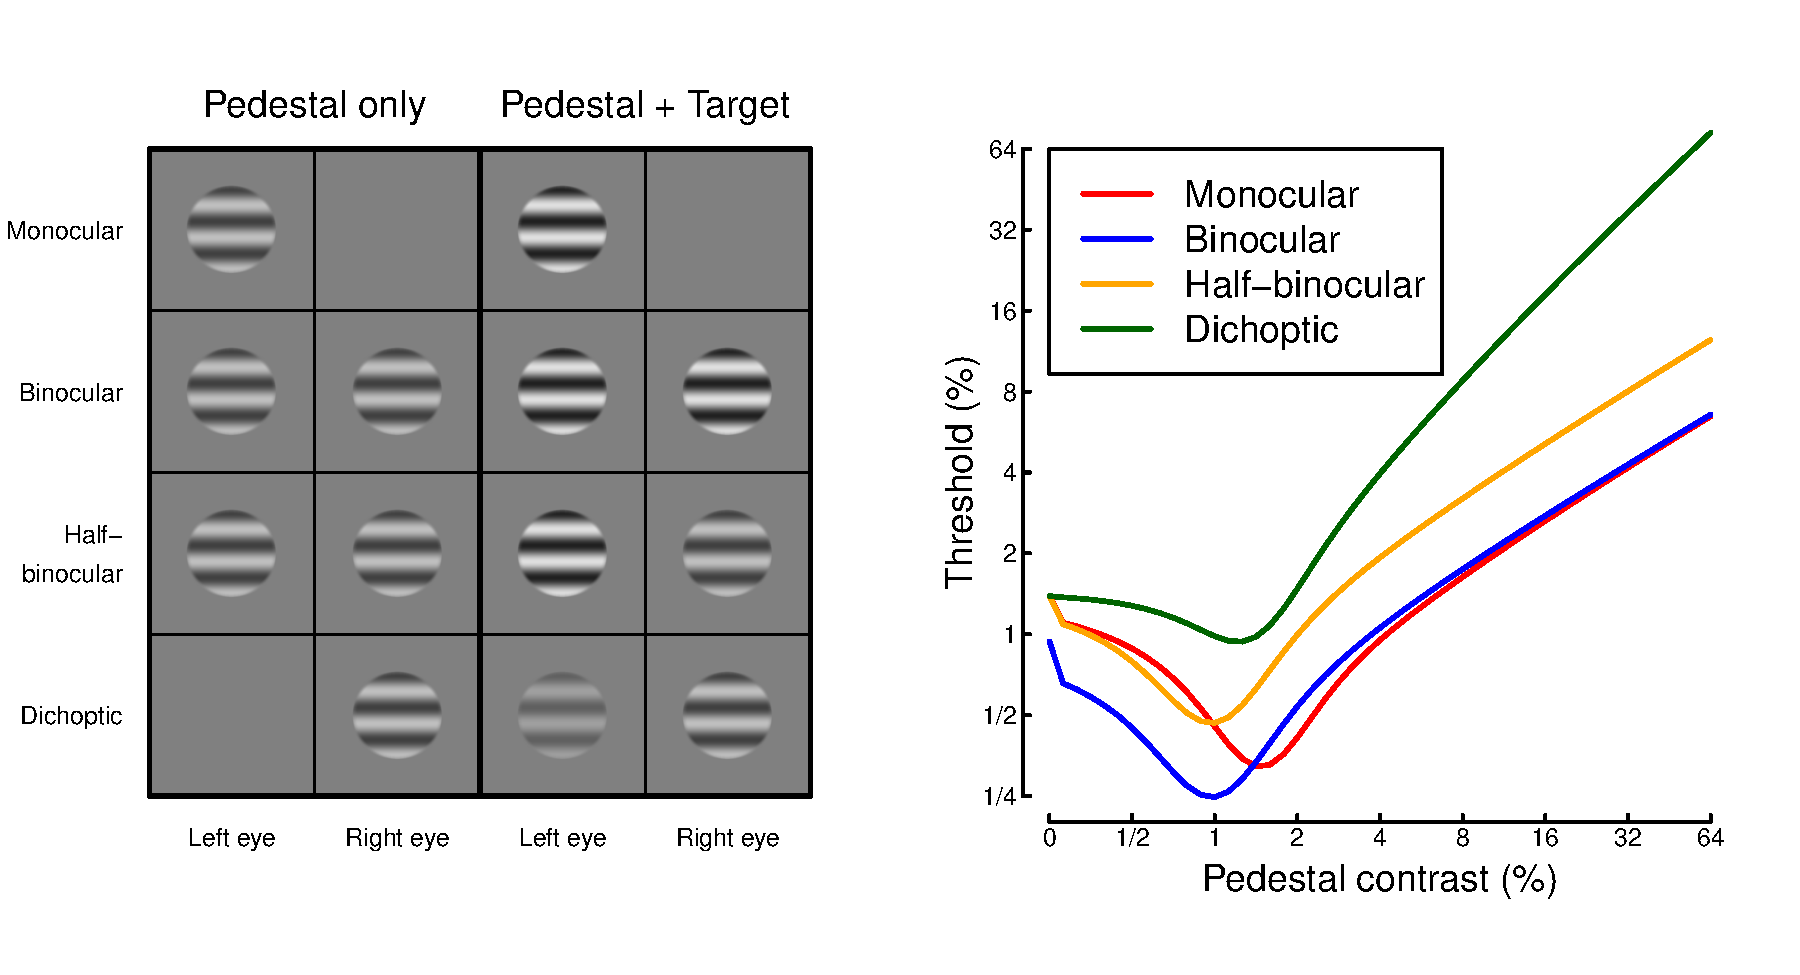
\includegraphics{Figures/exampledips} 

}

\caption{Illustration of stimulus conditions (left) and example dipper functions (right).}\label{fig:exampledips}
\end{figure}

The detailed pattern of results across these four conditions is complex, and for achromatic stimuli has several distinctive features that have been replicated in multiple studies. At low pedestal contrasts, the binocular condition yields lower thresholds than the monocular condition owing to binocular summation (Baker et al., 2018; Campbell \& Green, 1965). However at high pedestal contrasts the `handle' regions of the dipper functions for these conditions converge: a consequence of interocular suppression compensating for the increased excitation during binocular stimulation (Legge, 1984; Maehara \& Goryo, 2005). The half-binocular condition avoids confounding the number of eyes seeing the target with the number of eyes seeing the pedestal (Meese et al., 2006). The pedestal is always binocular in this condition, whereas the target increment is monocular, and thresholds are consistently higher than in the binocular condition across the full range of pedestal contrasts. This demonstrates that binocular summation occurs across the full contrast range, when the pedestal ocularity is appropriately controlled. Finally, the dichoptic condition produces extremely strong masking of the target, such that when the pedestal is visible, the target must equal or exceed its contrast in order to be detectable (Baker \& Meese, 2007; Legge, 1979; Maehara \& Goryo, 2005).

At the output of the human retina, visual signals are split into three chromatic pathways. The sum of long- and medium-wavelength cone outputs (L+M) transmits luminance information, and is likely responsible for the binocular combination effects previously studied using achromatic stimuli (see above). The difference of long- and medium-wavelength cone outputs (L-M) is responsive to chromatic stimuli modulating along a red/green axis in colour space. Finally the short wavelength cone outputs (S-(L+M)) code chromatic stimuli modulating along a blue/yellow axis. There has not yet been a detailed investigation of binocular contrast discrimination in either of these chromatic pathways, however there is reason to believe they may differ from the achromatic pathway. At detection threshold, binocular summation is greater for chromatic versus achromatic stimuli (Simmons, 2005), implying a more linear initial stage of processing. For cross-orientation masking, there are differences in the magnitude of masking between chromatic (red/green) and achromatic stimuli (Kim et al., 2013; Medina \& Mullen, 2009), as well as differences in their temporal dynamics (Kim \& Mullen, 2015). There are also interactions between chromatic and achromatic pathways both within (Chen et al., 2000) and between (Kingdom \& Libenson, 2015; Mullen et al., 2014) the eyes, yet these have not been fully explored for arrangements where the target and mask have the same orientation. Finally, the neurophysiological underpinnings of colour vision are distinct from the achromatic system. In primary visual cortex (V1), chromatic signals are processed in `blob' regions that are revealed by cytochrome oxidase staining (Horton \& Hubel, 1981). The blob regions appear to be largely monocular (Livingstone \& Hubel, 1984), suggesting that binocular combination for chromatic stimuli might occur later than for achromatic stimuli and be subject to different constraints.

Strong interocular normalization is well-established when using DC-balanced periodic stimuli such as sine-wave gratings (Baker \& Wade, 2017; Meese et al., 2006; Moradi \& Heeger, 2009). However there is some evidence that binocular combination is more linear for luminance increments (Anstis \& Ho, 1998; Levelt, 1965), particularly against a dark background (Baker et al., 2012). Our recent work has extended this finding to flickering discs of luminance, which are DC-balanced across time (Segala et al., 2023). Steady-state EEG responses from early visual cortex and psychophysical contrast matching data were both consistent with weak interocular suppression when using this stimulus arrangement, indicating that binocular combination rules may differ for temporal contrast.

The main aim of the present study is to characterise binocular signal combination for chromatic stimuli, and for temporal modulations of luminance. We also aimed to investigate interocular suppression between chromatic and achromatic pathways. We therefore preregistered a series of psychophysical experiments (see: \url{https://osf.io/3vdga/}). In Experiment 1 we replicate the four key pedestal masking conditions of Meese et al. (2006) described above for achromatic grating stimuli, and extend this to both red/green and blue/yellow isoluminant chromatic stimuli. In Experiment 2 we explore dichoptic masking within and between these stimuli. Experiment 3 repeats the achromatic condition from the first experiment, but using a temporally modulated disc rather than sine-wave gratings. We take a Bayesian approach to data analysis and modelling; by fitting a hierarchical version of the two-stage gain control model (Meese et al., 2006) we compare posterior parameter distributions to understand how model parameters such as the weight of interocular suppression vary across visual pathways.

\hypertarget{materials-methods}{%
\section{Materials \& Methods}\label{materials-methods}}

\hypertarget{participants}{%
\subsection{Participants}\label{participants}}

All experiments were completed by the first author (DHB) and two other participants, who differed for each experiment. Written informed consent was obtained before data collection began, and all procedures were approved by the ethics committee of the Department of Psychology at the University of York (ID number 2202).

\hypertarget{apparatus-stimuli}{%
\subsection{Apparatus \& stimuli}\label{apparatus-stimuli}}

In Experiments 1 and 2, the stimuli were horizontal sinusoidal gratings with a spatial frequency of 1c/deg. The gratings were windowed by a raised cosine envelope with a diameter of 3 degrees. Spatial phase, relative to a central fixation cross, was randomised on each trial across the four cardinal phases. In the achromatic conditions, the sine-wave modulated all three colour channels equally. In the L-M condition, we generated isoluminant stimuli for each participant (see Procedures) designed to maximise contrast between L and M cones, whilst keeping S cone activity constant. In the S-(L+M) condition, the isoluminant stimuli maximised S-cone contrast. Stimuli were converted from cone space to monitor RGB coordinates using the monitor spectral readings and the Stockman-Sharpe 2 degree cone fundamentals (Stockman \& Sharpe, 2000). The stimuli in Experiment 3 were temporal modulations of luminance, using the same raised cosine envelope as described above, but with no further spatial modulation. The stimuli counterphase flickered sinusoidally at 4Hz. In all experiments, we displayed a binocular fusion lock, consisting of three concentric rings of small square elements with random colour. A black central fixation cross was also displayed throughout.

All stimuli were presented on an Iiyama VisionMaster Pro 510 CRT monitor, with a refresh rate of 100Hz, and a resolution of 1024 x 768 pixels. The display was driven by a ViSaGe MkII stimulus generator (Cambridge Research Systems Ltd., Kent, UK) running in 42-bit colour mode (14 bits per colour channel). We presented stimuli to the left and right eyes independently using a four-mirror stereoscope with front-silvered mirrors. The display was luminance calibrated using a ColourCal photometer (Cambridge Research Systems), and gamma corrected by fitting a four-parameter gamma function to the output of each CRT gun. The maximum luminance was 87 cd/m\(^2\). We also measured the spectral output of each phosphor using a Jaz spectroradiometer (Ocean Insight, Florida), and used these measurements to convert between LMS (cone) space and the monitor RGB coordinates.

For convenience, we express stimulus contrast as a percentage of the maximum possible contrast that could be displayed on our system. For achromatic stimuli, the maximum contrast is 1, so this is equivalent to the standard Michelson contrast expressed as a percentage. For the isoluminant chromatic stimuli, the maximum displayable L-M (red/green) cone contrast was 0.1, and the maximum displayable S-(L+M) (blue/yellow) cone contrast was 0.88. So an L-M threshold of 50\% is a cone contrast of \(0.5\times0.1 = 0.05\), and an S-(L+M) threshold of 50\% is a cone contrast of \(0.5\times0.88 = 0.44\). The threshold values reported throughout can therefore be converted to cone contrast by a straightforward multiplicative transform.

\hypertarget{procedure}{%
\subsection{Procedure}\label{procedure}}

All experiments took place in a darkened room. Participants placed their heads in a chin rest mounted on a height-adjustable table, to which the stereoscope was also attached. The total optical viewing distance (including the light path through the mirrors) was XXcm, at which distance 1 degree of visual angle encompassed 48 pixels on the monitor.

Before beginning primary data collection, each participant in Experiments 1 and 2 completed an isoluminance adjustment task. Stimuli were presented that counterphase flickered at 5Hz, defined about either the L-M or S-(L+M) plane in cone space. Participants used a trackball to dynamically adjust the angle of the stimulus to minimise the percept of flicker. Each participant completed ten such trials for each colour plane, and the average angle across repetition was taken as the isoluminant point, and used to generate stimuli for the main experiment for that participant. Settings were very similar across participants for the S-(L+M) direction, and somewhat more heterogeneous for the L-M direction (see Figure \ref{fig:isofig}).

\begin{figure}

{\centering 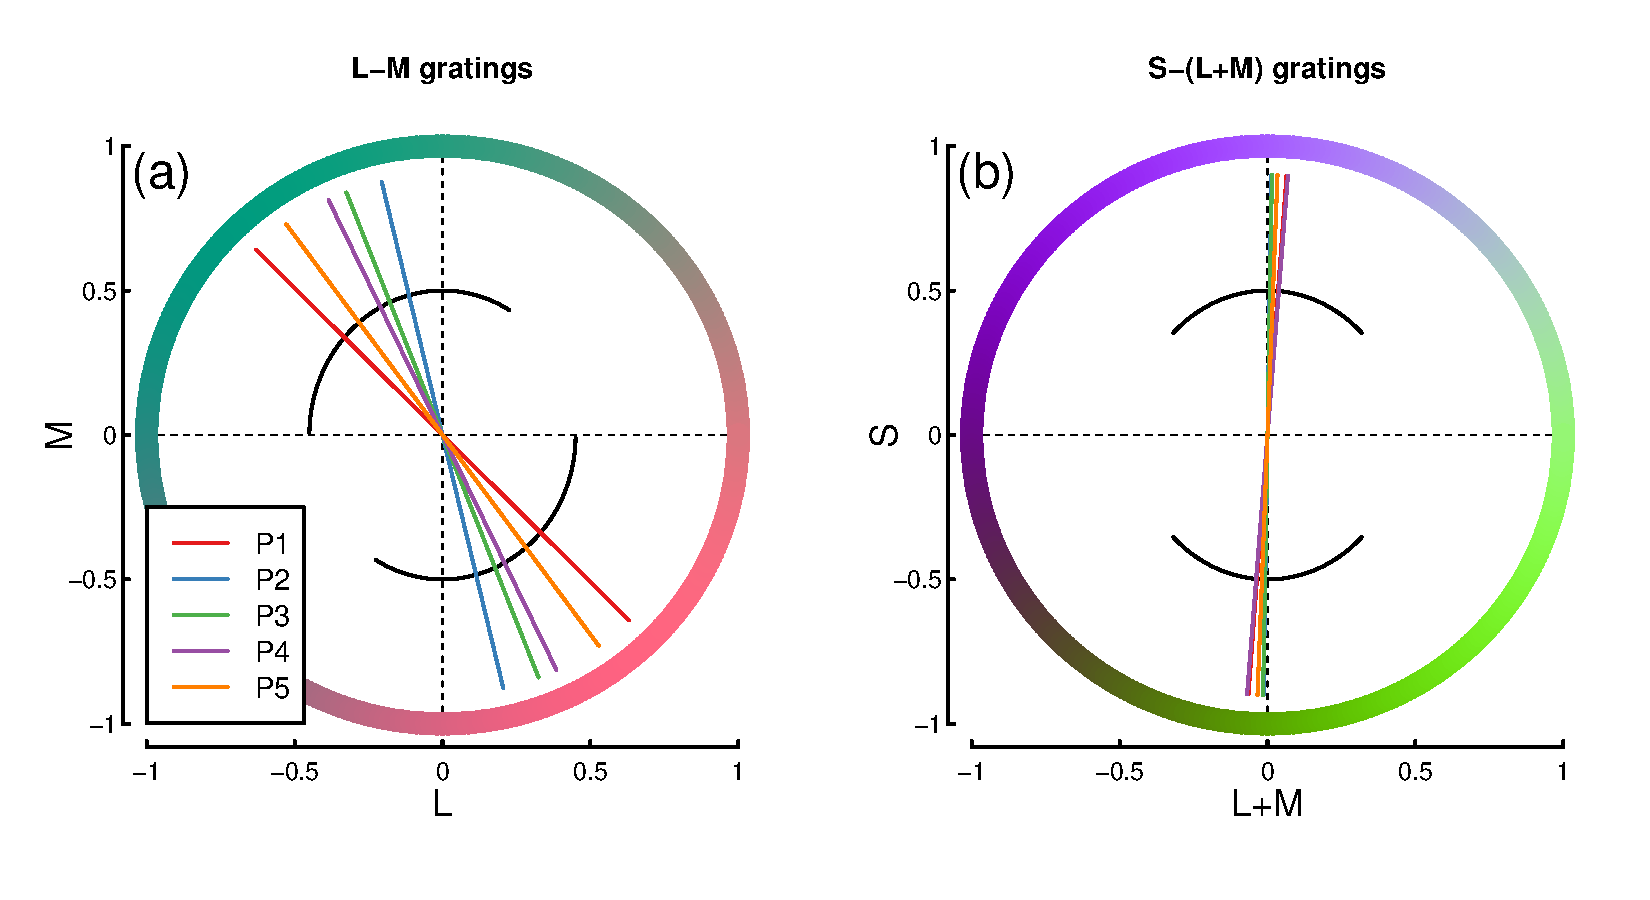
\includegraphics{Figures/isosettings} 

}

\caption{Isoluminance settings from all participants in Experiments 1 and 2. Panel (a) shows red/green and panel (b) shows blue/yellow settings that were subsequently used to generate stimuli in the main experiments. Within each panel, solid lines show the mean settings for each participant, and black curves show the range of possible stimuli displayed during the adjustment task.}\label{fig:isofig}
\end{figure}

In Experiment 1, participants completed a two-interval-forced-choice (2IFC) contrast discrimination task. Stimuli were presented for 200ms, with an interstimulus interval of 400ms. Each interval was indicated by an auditory beep, and participants made their responses using a two-button trackball. Correct trials were indicated by a high pitched tone, and incorrect trials by a low pitched tone. Each block of the experiment tested a single pedestal contrast level, and lasted around 12 minutes. On each trial the target contrast level was determined by a 3-down-1-up staircase procedure. There were 8 interleaved staircases in total; four stimulus arrangements (see Figure \ref{fig:exampledips}) by two target eye assignments. Each pedestal contrast was repeated 3 times by each participant, and the block order was randomised. The experiment lasted around 4 hours per participant for each chromatic condition, which took place over the course of several weeks. In total, the experiment consisted of 67978 trials (pooled across participants).

In Experiment 2, participants completed a 2IFC dichoptic masking task. The stimuli and trial protocol were the same as for Experiment 1, except that the target contrast was chosen from a set of 10 possible values, determined in advance based on the data of Experiment 1. There were 12 possible conditions: baseline detection thresholds for achromatic, red/green and blue/yellow stimuli, and the nine possible factorial pairings obtained by assigning these conditions to be target and dichoptic mask stimuli. Mask contrasts were chosen to be approximately 16 times their (monocular) detection threshold, based on the data from Experiment 1. Each block of the experiment tested a single condition, and consisted of 200 trials. A high contrast example of the target stimulus was displayed at the foot of the screen throughout, so that there was no ambiguity about the target identity on a given block. Participants completed 10 repetitions of each condition (120 blocks of \textasciitilde6 minutes each), lasting around 12 hours, for a total of 72000 trials (pooled across participants).

In Experiment 3, the achromatic conditions from Experiment 1 were repeated using a flickering disc stimulus. The stimulus counterphase flickered at 4Hz, and was presented for 500ms (i.e.~2 full cycles of the temporal modulation). All other procedures were the same as for Experiment 1, and the experiment comprised a total of X trials (pooled across participants).

\hypertarget{data-analysis-and-computational-modelling}{%
\subsection{Data analysis and computational modelling}\label{data-analysis-and-computational-modelling}}

Psychometric functions from each experiment were fit using \emph{psignifit} 4 to estimate full posterior distributions for threshold and slope parameters via a Bayesian numerical integration method (Schütt et al., 2016), fitting a cumulative Gaussian. We also implemented a Bayesian hierarchical version of the two stage model of Meese et al. (2006) using the Stan language (Carpenter et al., 2017). This used a binomial generator function to model the proportion correct data at each target level, and was fit separately to each chromatic condition of Experiment 1, and the data of Experiment 3 (i.e.~4 model fits in total). The modelling primarily focuses on comparing posterior parameter distributions across conditions and experiments, rather than a model comparison approach. We generated over 1 million posterior samples for each model, and retained 10\% of them for plotting.

\hypertarget{open-science-practices}{%
\subsection{Open science practices}\label{open-science-practices}}

All experimental code, raw data and analysis scripts are available at: \url{https://osf.io/3vdga/}. The linked GitHub repository also contains a fully reproducible version of the manuscript. Note that we deviated slightly from the planned preregistration, in that we did not collect data for chromatic flickering discs, or for the cross-pathway dichoptic experiment using disc stimuli. This is because the grating data from Experiments 1 and 2, and the achromatic disc data from Experiment 3, were sufficient to address the questions we had wanted to answer from these experiments.

\hypertarget{results}{%
\section{Results}\label{results}}

\hypertarget{experiment-1}{%
\subsection{Experiment 1}\label{experiment-1}}

Dipper functions from Experiment 1 are displayed in Figure \ref{fig:dipperfig}. Panel (a) shows the achromatic results, which replicate the key features from previous work. At detection threshold, binocular summation was a factor of 1.67 (4.47dB), consistent with previous reports. Pedestal masking functions follow the typical `dipper' shape in all conditions, with a region of facilitation at low pedestal contrasts, and masking at higher contrasts. The monocular and binocular dipper handles converge at high contrasts, whereas the half-binocular thresholds remain above the binocular thresholds across the full range of pedestal contrasts. The dichoptic condition produced very high thresholds, with the rising portion of the dipper having a slope around 1 (regression slope of 1.06 across the highest 4 pedestal contrasts in log (dB) units).

\begin{figure}

{\centering 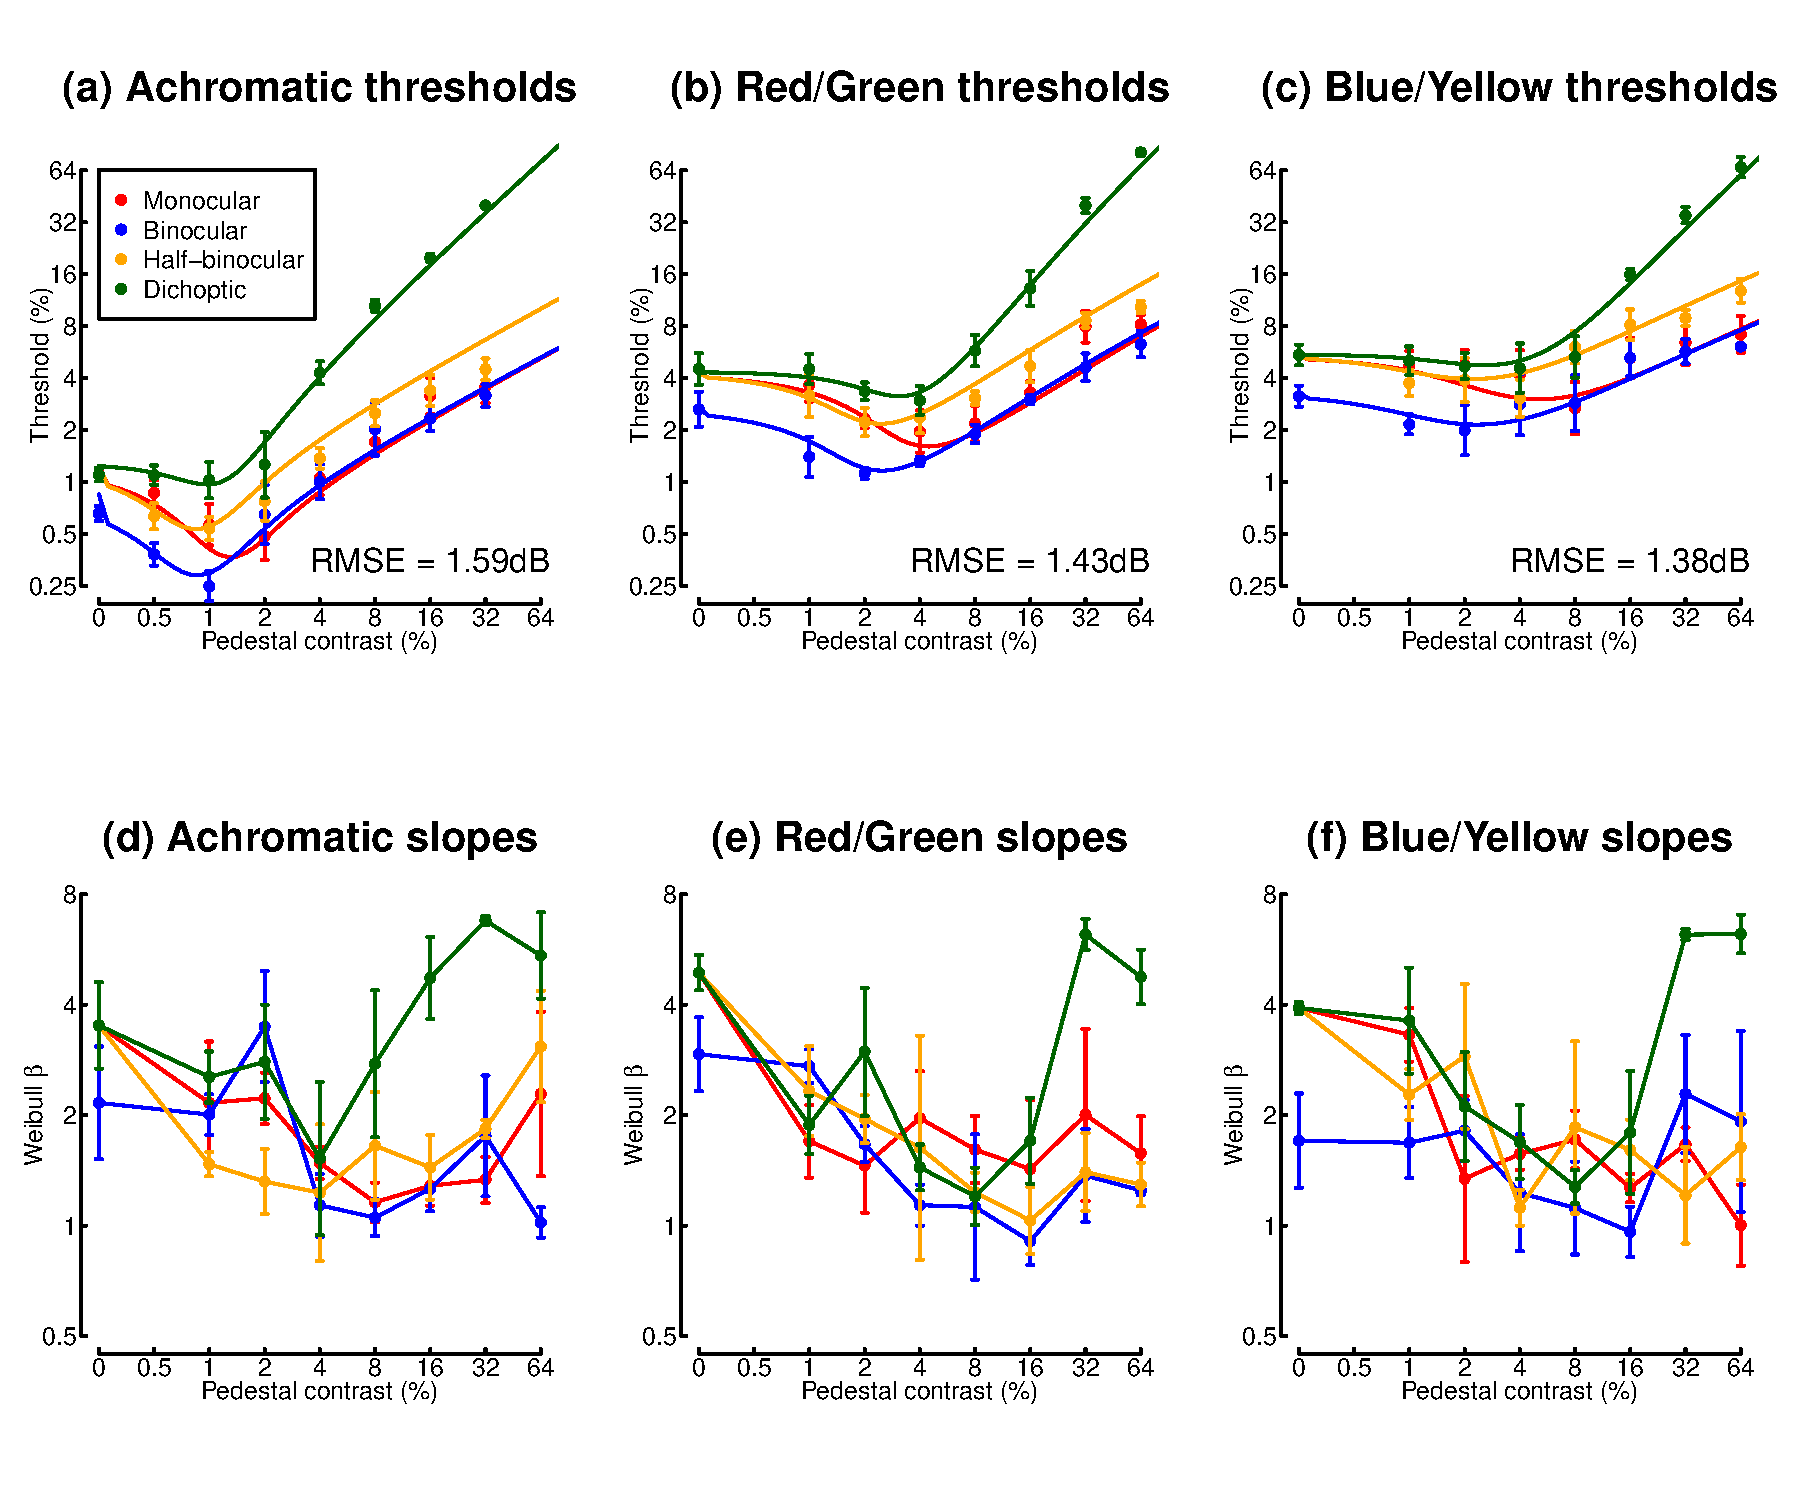
\includegraphics{Figures/dipperssimplex} 

}

\caption{Dipper functions from Experiment 1, averaged across three participants. Error bars show ±1SE across participants. Note that contrast values are expressed as a percentage of the maximum displayable contrast (see Procedures for details).}\label{fig:dipperfig}
\end{figure}

A similar pattern of results was observed for both the red/green and blue/yellow isoluminant stimuli (see Figure \ref{fig:dipperfig}b,c). Summation at threshold was a factor of 1.71 (4.66dB) for the red/green targets, and a factor of 1.73 (4.77dB) for the blue/yellow targets, and so was marginally higher than for achromatic stimuli. The general character of the dipper functions was largely consistent with the achromatic results, though we observed shallower facilitation and weaker masking, especially for the blue/yellow stimuli. For example, the strongest facilitation in the binocular condition for achromatic stimuli was a factor of 2.63, whereas it reduced to a factor of 2.35 for red/green stimuli and 1.57 for blue/yellow stimuli. The slope of the binocular dipper handle was 0.52 for achromatic stimuli, 0.58 for red/green stimuli, and 0.34 for blue/yellow stimuli. Dichoptic masking remained as strong for the chromatic conditions as for the achromatic stimuli (regression slopes of 1.3 for red/green and 1.21 for blue/yellow). The pattern of results for individual participants was consistent with the averages, as shown in Figure \ref{fig:individualdips}.

Modelling

\begin{figure}

{\centering 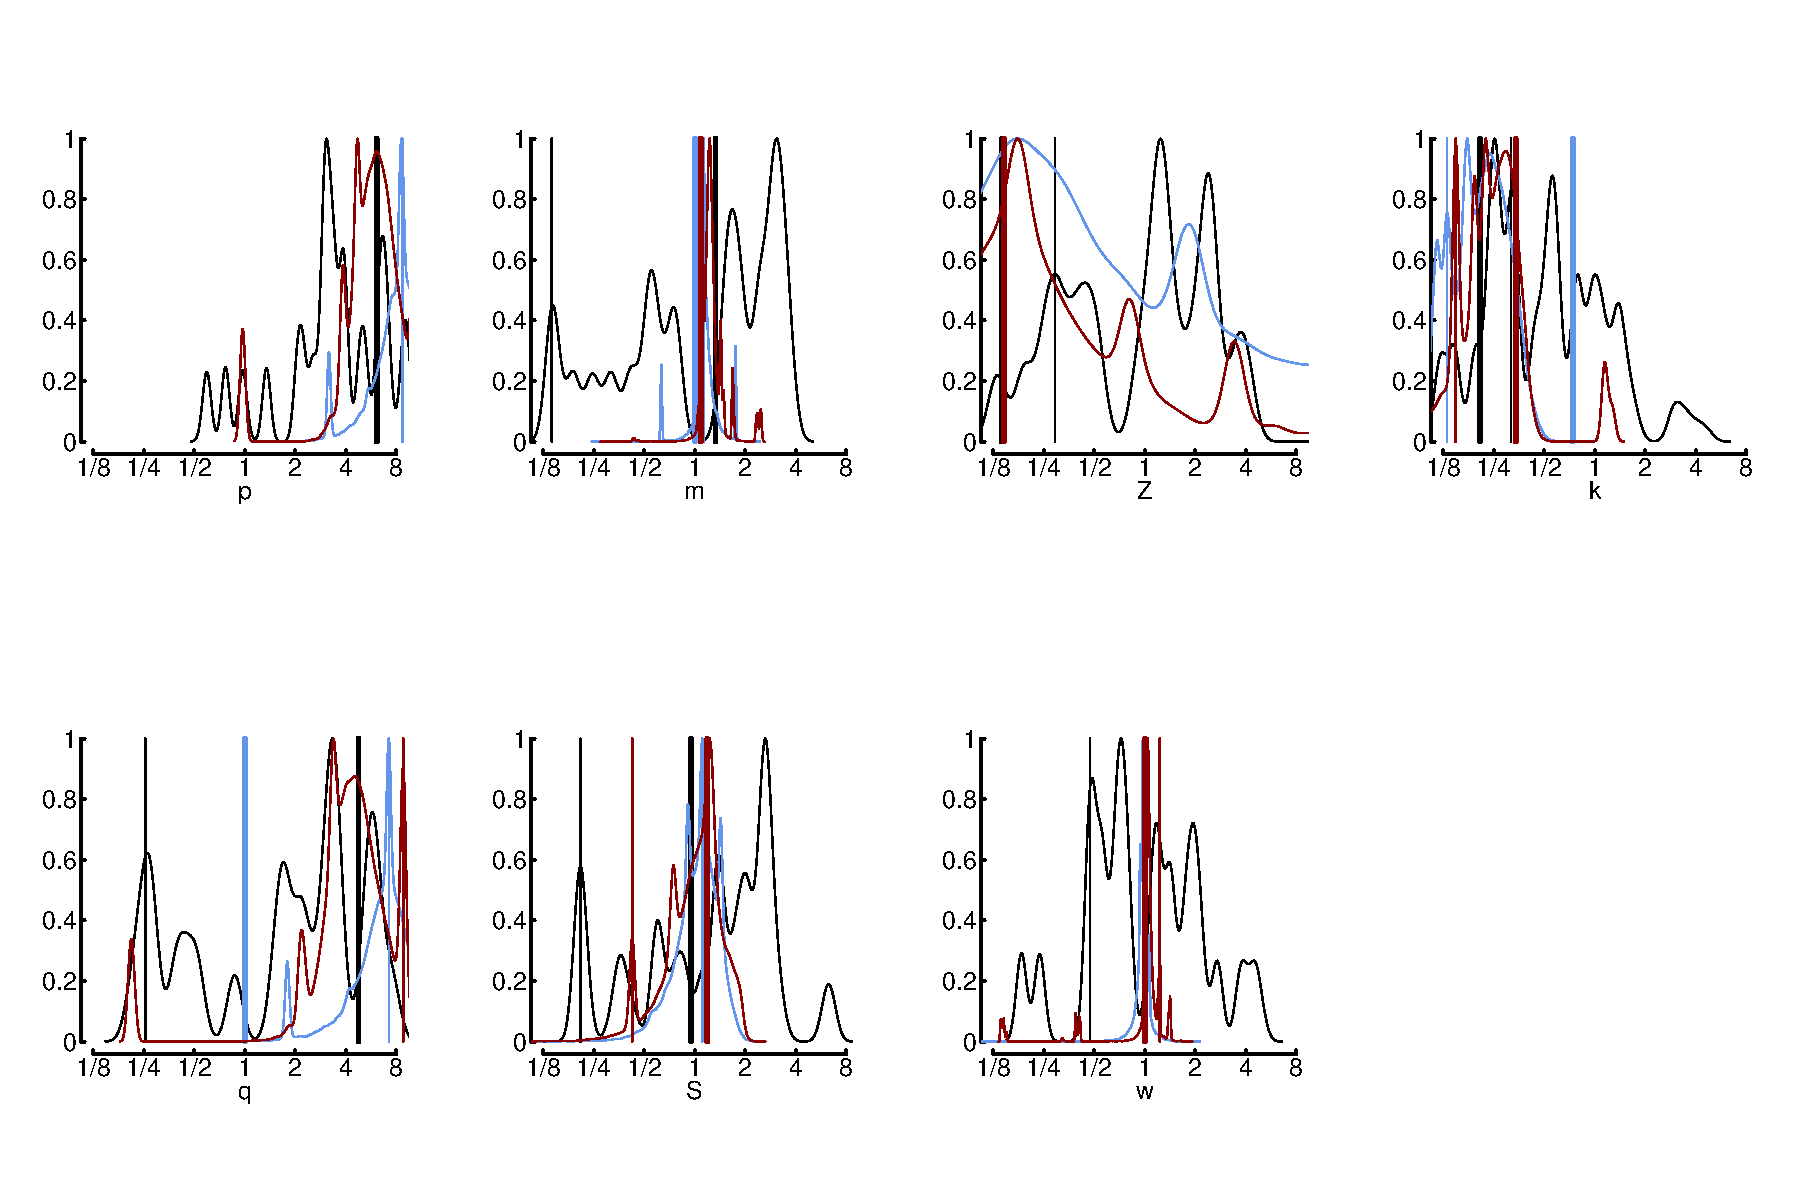
\includegraphics{Figures/modelparams} 

}

\caption{Model parameters}\label{fig:params}
\end{figure}

\hypertarget{experiment-2}{%
\subsection{Experiment 2}\label{experiment-2}}

In Experiment 2 we focussed on the dichoptic condition at a single mask contrast, and measured full psychometric functions using the method of constant stimuli for all factorial pairings of target and mask chromaticity. The pooled results across three participants are shown in Figure \ref{fig:MCSfig}, and results for individual participants are available in Figure \ref{fig:individualMCS}. All conditions produced monotonically increasing psychometric functions (panels a-c), but the extent of masking was highly dependent on the relationship between the target and mask chromaticity.

\begin{figure}

{\centering 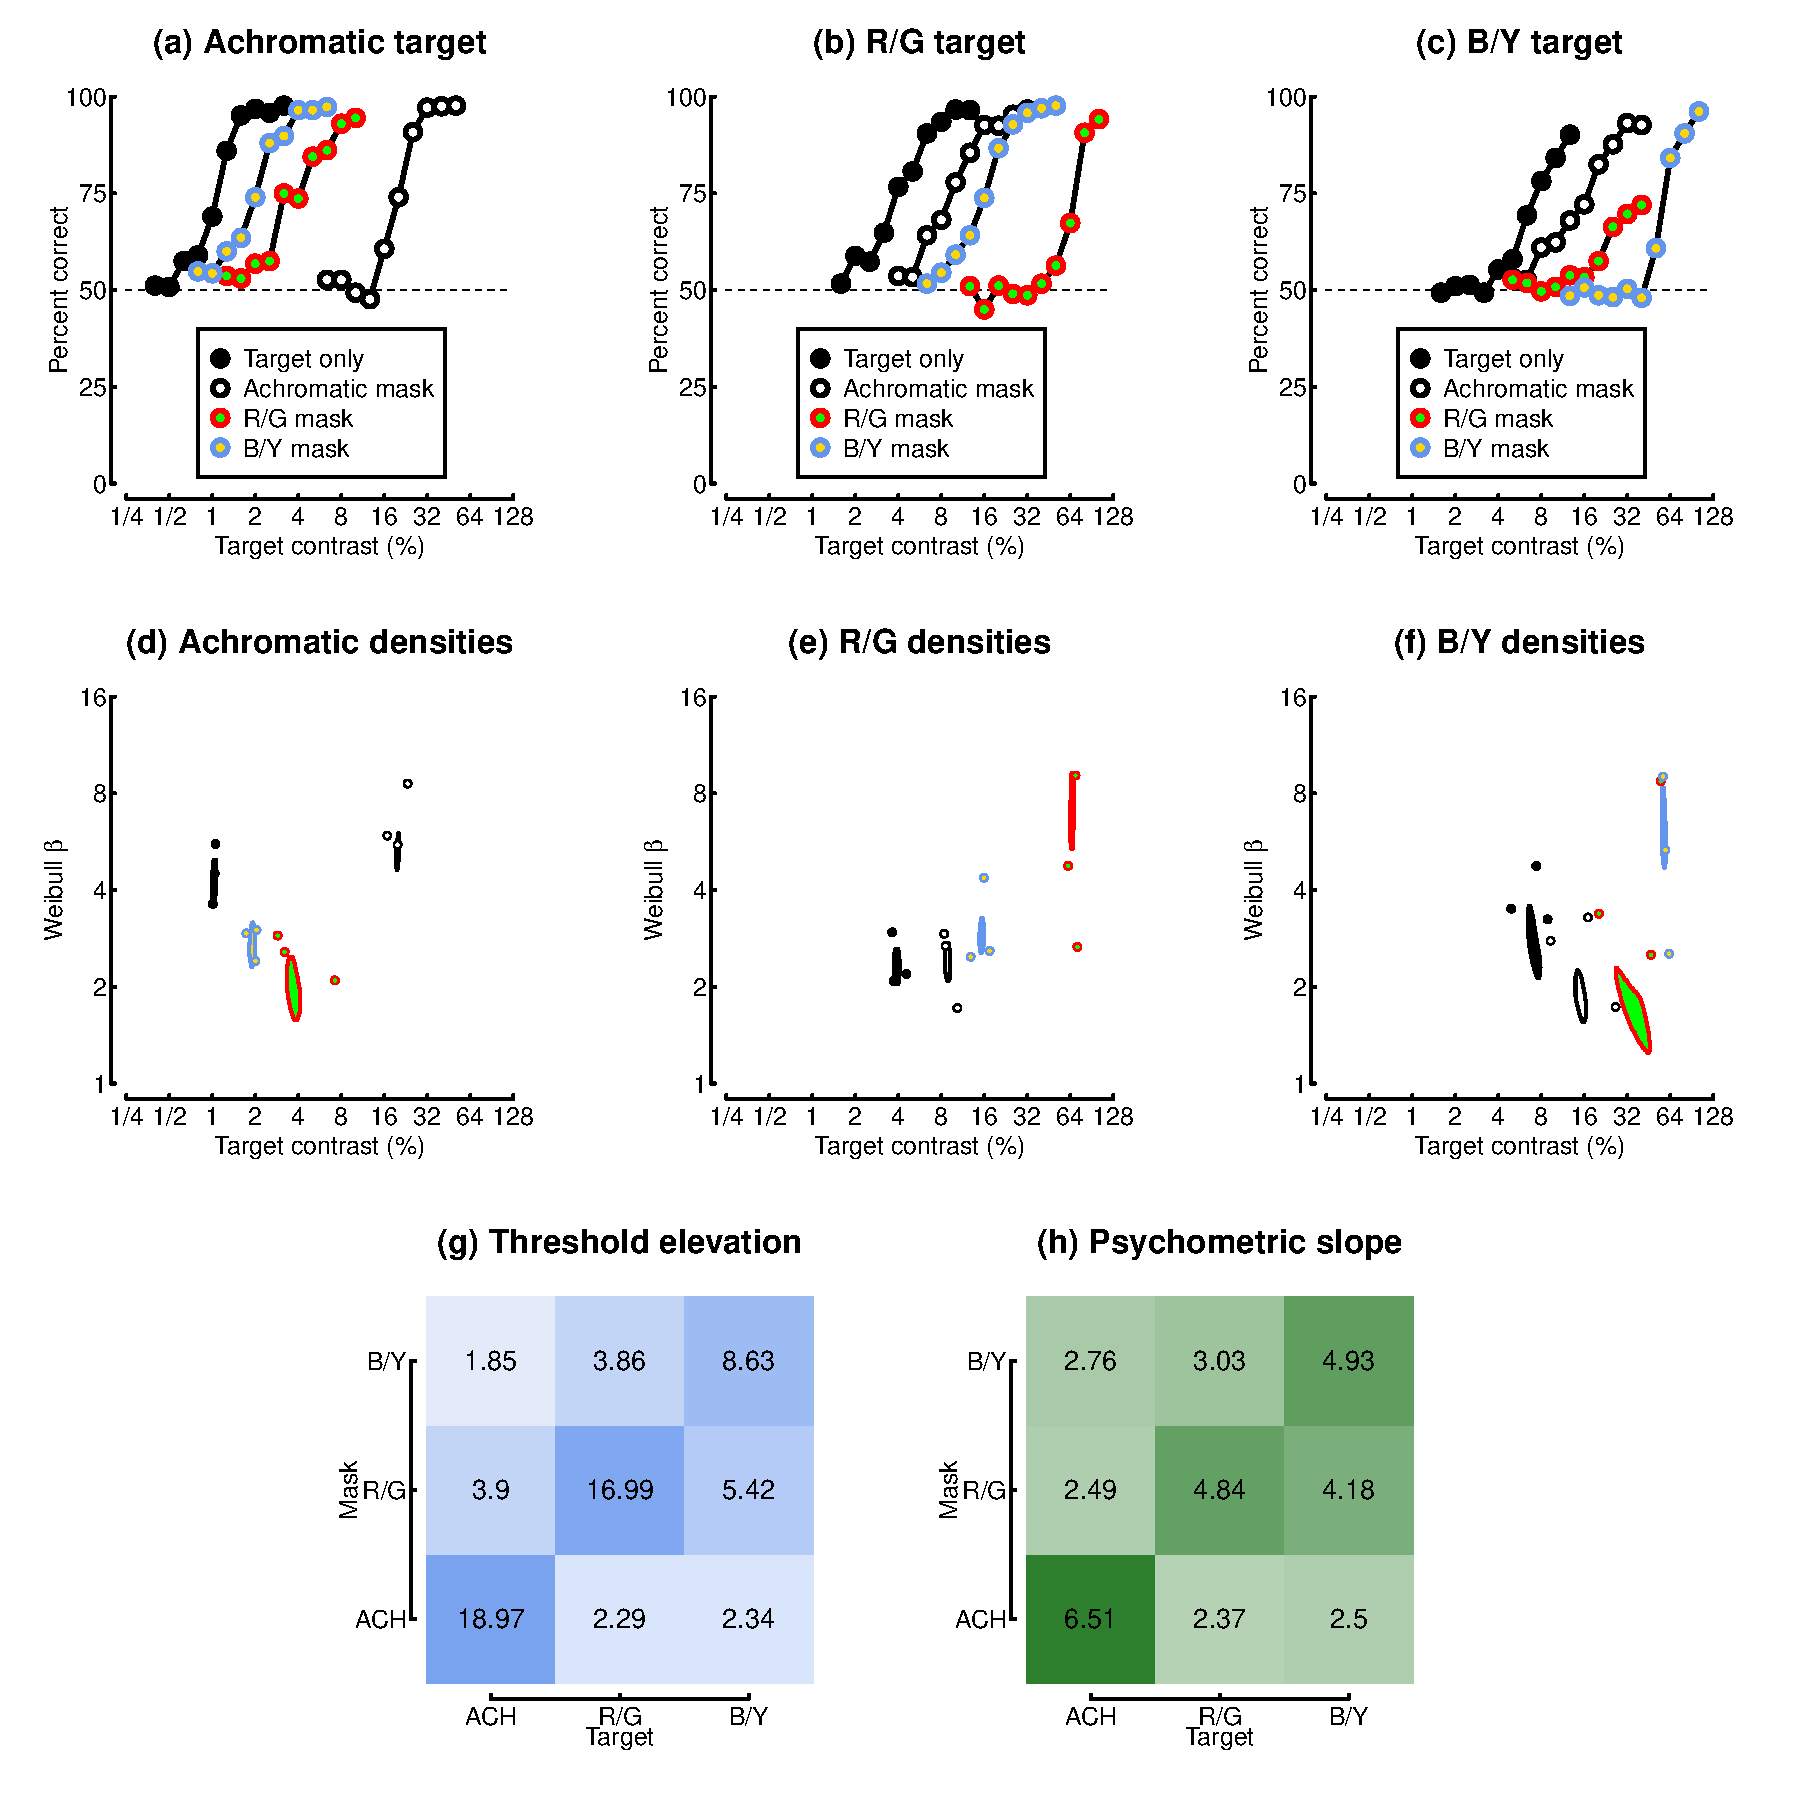
\includegraphics{Figures/MCSdata} 

}

\caption{Summary of data from Experiment 2. Panels (a-c) show psychometric functions for each condition, pooled across participants (600 trials per target contrast level). Panel (d) shows the average threshold elevation factor for each combination of target and mask stimulus. Panel (e) shows the geometric mean psychometric slope value for each masking condition in Weibull beta units.}\label{fig:MCSfig}
\end{figure}

Threshold elevation was greatest when the target and mask had the same chromaticity - notice that the psychometric function is shifted furthest to the right for the achromatic target with an achromatic mask (white and black circles in Figure \ref{fig:MCSfig}a), for the red/green target with a red/green mask (red and green circles in Figure \ref{fig:MCSfig}b), and for the blue/yellow target with a blue/yellow mask (blue and yellow circles in Figure \ref{fig:MCSfig}c). Masking was weakest between achromatic masks/targets and chromatic masks/targets. Finally there was an intermediate level of masking between red/green and blue/yellow stimuli. This is summarised in Figure \ref{fig:MCSfig}d, which represents threshold elevation for each combination of target and mask chromaticity. Note that the positive diagonal exhibits the highest values, and represents threshold elevation between targets and masks of the same chromaticity.

We also calculated the slope of the psychometric function for each condition, converted to equivalent Weibull \(\beta\) values. In the absence of a mask, the average slope was \(\beta\) = 3.42, which is typical for contrast detection tasks. Slopes became substantially steeper when the dichoptic mask matched the target in chromaticity (average \(\beta\) = 5.38). These `super-steep' psychometric functions for dichoptic pedestal masking have been reported previously (Baker et al., 2013; Meese et al., 2006), and are observed for the first time here using chromatic stimuli (see diagonal values in Figure \ref{fig:MCSfig}e). However we did not see such markedly steep functions for any of the cross-chromaticity masking conditions (average \(\beta\) = 2.83 for the off-diagonal values).

\hypertarget{experiment-3}{%
\subsection{Experiment 3}\label{experiment-3}}

In our final experiment, we again measured dipper functions, but this time for a temporally modulating luminance disc. This was motivated by our recent work (Segala et al., 2023) that appeared to show increased binocular facilitation and reduced interocular suppression for flickering disc stimuli (relative to gratings), measured using EEG and a psychophysical matching paradigm. The pattern of dipper functions for a 4Hz flickering disc (see Figure X) was very similar to that observed for achromatic gratings (see Figure \ref{fig:dipperfig}a), and the binocular summation ratio at threshold was also similar (a factor of). Fitting the same computational model to the disc data also generated an estimated weight of interocular suppression around 1. Data for individual participants are shown in Figure AX.

\hypertarget{discussion}{%
\section{Discussion}\label{discussion}}

Across three psychophysical experiments, we have demonstrated that:

\begin{itemize}
\tightlist
\item
  Binocular combination of isoluminant chromatic stimuli is similar to that for achromatic stimuli
\item
  Interocular suppression is strongest within a chromatic pathway, and weakest between achromatic and chromatic pathways
\item
  Binocular combination occurs similarly for temporal and temporal luminance modulations
\end{itemize}

We now discuss the relationship to previous work, consider the likely physiological substrates of these effects and .

Recent evidence indicates that the physiological substrate of interocular suppression may be neurons in layer 4 of primary visual cortex (Dougherty et al., 2019). Most cells in this layer are monocularly exciteable, in that their responses increase only by stimulation of their preferred eye. However, simultaneous stimulation of the non-preferred eye can modulate the response, usually in an inhibitory fashion, exactly as proposed by the two-stage model. In terms of perception, the consequence of this early suppression is to achieve `ocularity invariance', whereby the perceived contrast of a stimulus viewed by one eye is equivalent to that of the same stimulus viewed by both eyes (Baker et al., 2007). Similar processes of invariance have also been reported using fMRI (Moradi \& Heeger, 2009) and steady-state EEG (Baker \& Wade, 2017).

\hypertarget{conclusions}{%
\section{Conclusions}\label{conclusions}}

\hypertarget{acknowledgements}{%
\section{Acknowledgements}\label{acknowledgements}}

Supported by BBSRC grant BB/V007580/1 awarded to DHB and ARW.

\hypertarget{references}{%
\section{References}\label{references}}

\hypertarget{refs}{}
\begin{CSLReferences}{1}{0}
\leavevmode\vadjust pre{\hypertarget{ref-Anstis1998}{}}%
Anstis, S., \& Ho, A. (1998). Nonlinear combination of luminance excursions during flicker, simultaneous contrast, afterimages and binocular fusion. \emph{Vision Res}, \emph{38}(4), 523--539. \url{https://doi.org/10.1016/s0042-6989(97)00167-3}

\leavevmode\vadjust pre{\hypertarget{ref-Baker2018}{}}%
Baker, D. H., Lygo, F. A., Meese, T. S., \& Georgeson, M. A. (2018). Binocular summation revisited: Beyond \(\sqrt{2}\). \emph{Psychol Bull}, \emph{144}(11), 1186--1199. \url{https://doi.org/10.1037/bul0000163}

\leavevmode\vadjust pre{\hypertarget{ref-Baker2007b}{}}%
Baker, D. H., \& Meese, T. S. (2007). Binocular contrast interactions: Dichoptic masking is not a single process. \emph{Vision Res}, \emph{47}(24), 3096--3107. \url{https://doi.org/10.1016/j.visres.2007.08.013}

\leavevmode\vadjust pre{\hypertarget{ref-Baker2007}{}}%
Baker, D. H., Meese, T. S., \& Georgeson, M. A. (2007). Binocular interaction: Contrast matching and contrast discrimination are predicted by the same model. \emph{Spat Vis}, \emph{20}(5), 397--413. \url{https://doi.org/10.1163/156856807781503622}

\leavevmode\vadjust pre{\hypertarget{ref-Baker2013}{}}%
Baker, D. H., Meese, T. S., \& Georgeson, M. A. (2013). Paradoxical psychometric functions ("swan functions") are explained by dilution masking in four stimulus dimensions. \emph{Iperception}, \emph{4}(1), 17--35. \url{https://doi.org/10.1068/i0552}

\leavevmode\vadjust pre{\hypertarget{ref-Baker2017}{}}%
Baker, D. H., \& Wade, A. R. (2017). Evidence for an optimal algorithm underlying signal combination in human visual cortex. \emph{Cereb Cortex}, \emph{27}(1), 254--264. \url{https://doi.org/10.1093/cercor/bhw395}

\leavevmode\vadjust pre{\hypertarget{ref-Baker2012}{}}%
Baker, D. H., Wallis, S. A., Georgeson, M. A., \& Meese, T. S. (2012). Nonlinearities in the binocular combination of luminance and contrast. \emph{Vision Res}, \emph{56}, 1--9. \url{https://doi.org/10.1016/j.visres.2012.01.008}

\leavevmode\vadjust pre{\hypertarget{ref-Campbell1965}{}}%
Campbell, F. W., \& Green, D. G. (1965). Monocular versus binocular visual acuity. \emph{Nature}, \emph{208}(5006), 191--192. \url{https://doi.org/10.1038/208191a0}

\leavevmode\vadjust pre{\hypertarget{ref-Carpenter2017}{}}%
Carpenter, B., Gelman, A., Hoffman, M. D., Lee, D., Goodrich, B., Betancourt, M., Brubaker, M., Guo, J., Li, P., \& Riddell, A. (2017). Stan: A probabilistic programming language. \emph{Journal of Statistical Software}, \emph{76}(1), 1--32. \url{https://doi.org/10.18637/jss.v076.i01}

\leavevmode\vadjust pre{\hypertarget{ref-Chen2000}{}}%
Chen, C., Foley, J. M., \& Brainard, D. H. (2000). Detection of chromoluminance patterns on chromoluminance pedestals i: Threshold measurements. \emph{Vision Res}, \emph{40}(7), 773--788. \url{https://doi.org/10.1016/s0042-6989(99)00227-8}

\leavevmode\vadjust pre{\hypertarget{ref-Dougherty2019}{}}%
Dougherty, K., Cox, M. A., Westerberg, J. A., \& Maier, A. (2019). Binocular modulation of monocular V1 neurons. \emph{Curr Biol}, \emph{29}(3), 381--391.e4. \url{https://doi.org/10.1016/j.cub.2018.12.004}

\leavevmode\vadjust pre{\hypertarget{ref-Georgeson2016}{}}%
Georgeson, M. A., Wallis, S. A., Meese, T. S., \& Baker, D. H. (2016). Contrast and lustre: A model that accounts for eleven different forms of contrast discrimination in binocular vision. \emph{Vision Res}, \emph{129}, 98--118. \url{https://doi.org/10.1016/j.visres.2016.08.001}

\leavevmode\vadjust pre{\hypertarget{ref-Horton1981}{}}%
Horton, J. C., \& Hubel, D. H. (1981). Regular patchy distribution of cytochrome oxidase staining in primary visual cortex of macaque monkey. \emph{Nature}, \emph{292}(5825), 762--764. \url{https://doi.org/10.1038/292762a0}

\leavevmode\vadjust pre{\hypertarget{ref-Kim2013}{}}%
Kim, Y. J., Gheiratmand, M., \& Mullen, K. T. (2013). Cross-orientation masking in human color vision: Application of a two-stage model to assess dichoptic and monocular sources of suppression. \emph{J Vis}, \emph{13}(6), 15. \url{https://doi.org/10.1167/13.6.15}

\leavevmode\vadjust pre{\hypertarget{ref-Kim2015}{}}%
Kim, Y. J., \& Mullen, K. T. (2015). The dynamics of cross-orientation masking at monocular and interocular sites. \emph{Vision Res}, \emph{116}(Pt A), 80--91. \url{https://doi.org/10.1016/j.visres.2015.09.008}

\leavevmode\vadjust pre{\hypertarget{ref-Kingdom2015}{}}%
Kingdom, F. A. A., \& Libenson, L. (2015). Dichoptic color saturation mixture: Binocular luminance contrast promotes perceptual averaging. \emph{J Vis}, \emph{15}(5), 2. \url{https://doi.org/10.1167/15.5.2}

\leavevmode\vadjust pre{\hypertarget{ref-Legge1979}{}}%
Legge, G. E. (1979). Spatial frequency masking in human vision: Binocular interactions. \emph{J Opt Soc Am}, \emph{69}(6), 838--847. \url{https://doi.org/10.1364/josa.69.000838}

\leavevmode\vadjust pre{\hypertarget{ref-Legge1984}{}}%
Legge, G. E. (1984). Binocular contrast summation--II. Quadratic summation. \emph{Vision Res}, \emph{24}(4), 385--394. \url{https://doi.org/10.1016/0042-6989(84)90064-6}

\leavevmode\vadjust pre{\hypertarget{ref-Levelt1965}{}}%
Levelt, W. J. (1965). Binocular brightness averaging and contour information. \emph{Br J Psychol}, \emph{56}, 1--13. \url{https://doi.org/10.1111/j.2044-8295.1965.tb00939.x}

\leavevmode\vadjust pre{\hypertarget{ref-Livingstone1984}{}}%
Livingstone, M. S., \& Hubel, D. H. (1984). Anatomy and physiology of a color system in the primate visual cortex. \emph{J Neurosci}, \emph{4}(1), 309--356. \url{https://doi.org/10.1523/JNEUROSCI.04-01-00309.1984}

\leavevmode\vadjust pre{\hypertarget{ref-Maehara2005}{}}%
Maehara, G., \& Goryo, K. (2005). Binocular, monocular and dichoptic pattern masking. \emph{Optical Review}, \emph{12}(2), 76--82. \url{https://doi.org/10.1007/PL00021542}

\leavevmode\vadjust pre{\hypertarget{ref-Medina2009}{}}%
Medina, J. M., \& Mullen, K. T. (2009). Cross-orientation masking in human color vision. \emph{J Vis}, \emph{9}(3), 20.1--16. \url{https://doi.org/10.1167/9.3.20}

\leavevmode\vadjust pre{\hypertarget{ref-Meese2006}{}}%
Meese, T. S., Georgeson, M. A., \& Baker, D. H. (2006). Binocular contrast vision at and above threshold. \emph{J Vis}, \emph{6}(11), 1224--1243. \url{https://doi.org/10.1167/6.11.7}

\leavevmode\vadjust pre{\hypertarget{ref-Moradi2009}{}}%
Moradi, F., \& Heeger, D. J. (2009). Inter-ocular contrast normalization in human visual cortex. \emph{J Vis}, \emph{9}(3), 13.1--22. \url{https://doi.org/10.1167/9.3.13}

\leavevmode\vadjust pre{\hypertarget{ref-Mullen2014}{}}%
Mullen, K. T., Kim, Y. J., \& Gheiratmand, M. (2014). Contrast normalization in colour vision: The effect of luminance contrast on colour contrast detection. \emph{Sci Rep}, \emph{4}, 7350. \url{https://doi.org/10.1038/srep07350}

\leavevmode\vadjust pre{\hypertarget{ref-Schutt2016}{}}%
Schütt, H. H., Harmeling, S., Macke, J. H., \& Wichmann, F. A. (2016). Painfree and accurate bayesian estimation of psychometric functions for (potentially) overdispersed data. \emph{Vision Res}, \emph{122}, 105--123. \url{https://doi.org/10.1016/j.visres.2016.02.002}

\leavevmode\vadjust pre{\hypertarget{ref-Segala2023}{}}%
Segala, F. G., Bruno, A., Martin, J. T., Aung, M. T., Wade, A. R., \& Baker, D. H. (2023). Different rules for binocular combination of luminance flicker in cortical and subcortical pathways. \emph{eLife}, \emph{12}, RP87048. \url{https://doi.org/10.7554/eLife.87048}

\leavevmode\vadjust pre{\hypertarget{ref-Simmons2005}{}}%
Simmons, D. R. (2005). The binocular combination of chromatic contrast. \emph{Perception}, \emph{34}(8), 1035--1042. \url{https://doi.org/10.1068/p5279}

\leavevmode\vadjust pre{\hypertarget{ref-Stockman2000}{}}%
Stockman, A., \& Sharpe, L. T. (2000). The spectral sensitivities of the middle- and long-wavelength-sensitive cones derived from measurements in observers of known genotype. \emph{Vision Res}, \emph{40}(13), 1711--1737. \url{https://doi.org/10.1016/s0042-6989(00)00021-3}

\end{CSLReferences}

\hypertarget{appendices}{%
\section{Appendices}\label{appendices}}

\setcounter{table}{0}  \renewcommand{\thetable}{A\arabic{table}} \setcounter{figure}{0} \renewcommand{\thefigure}{A\arabic{figure}}

\begin{figure}

{\centering 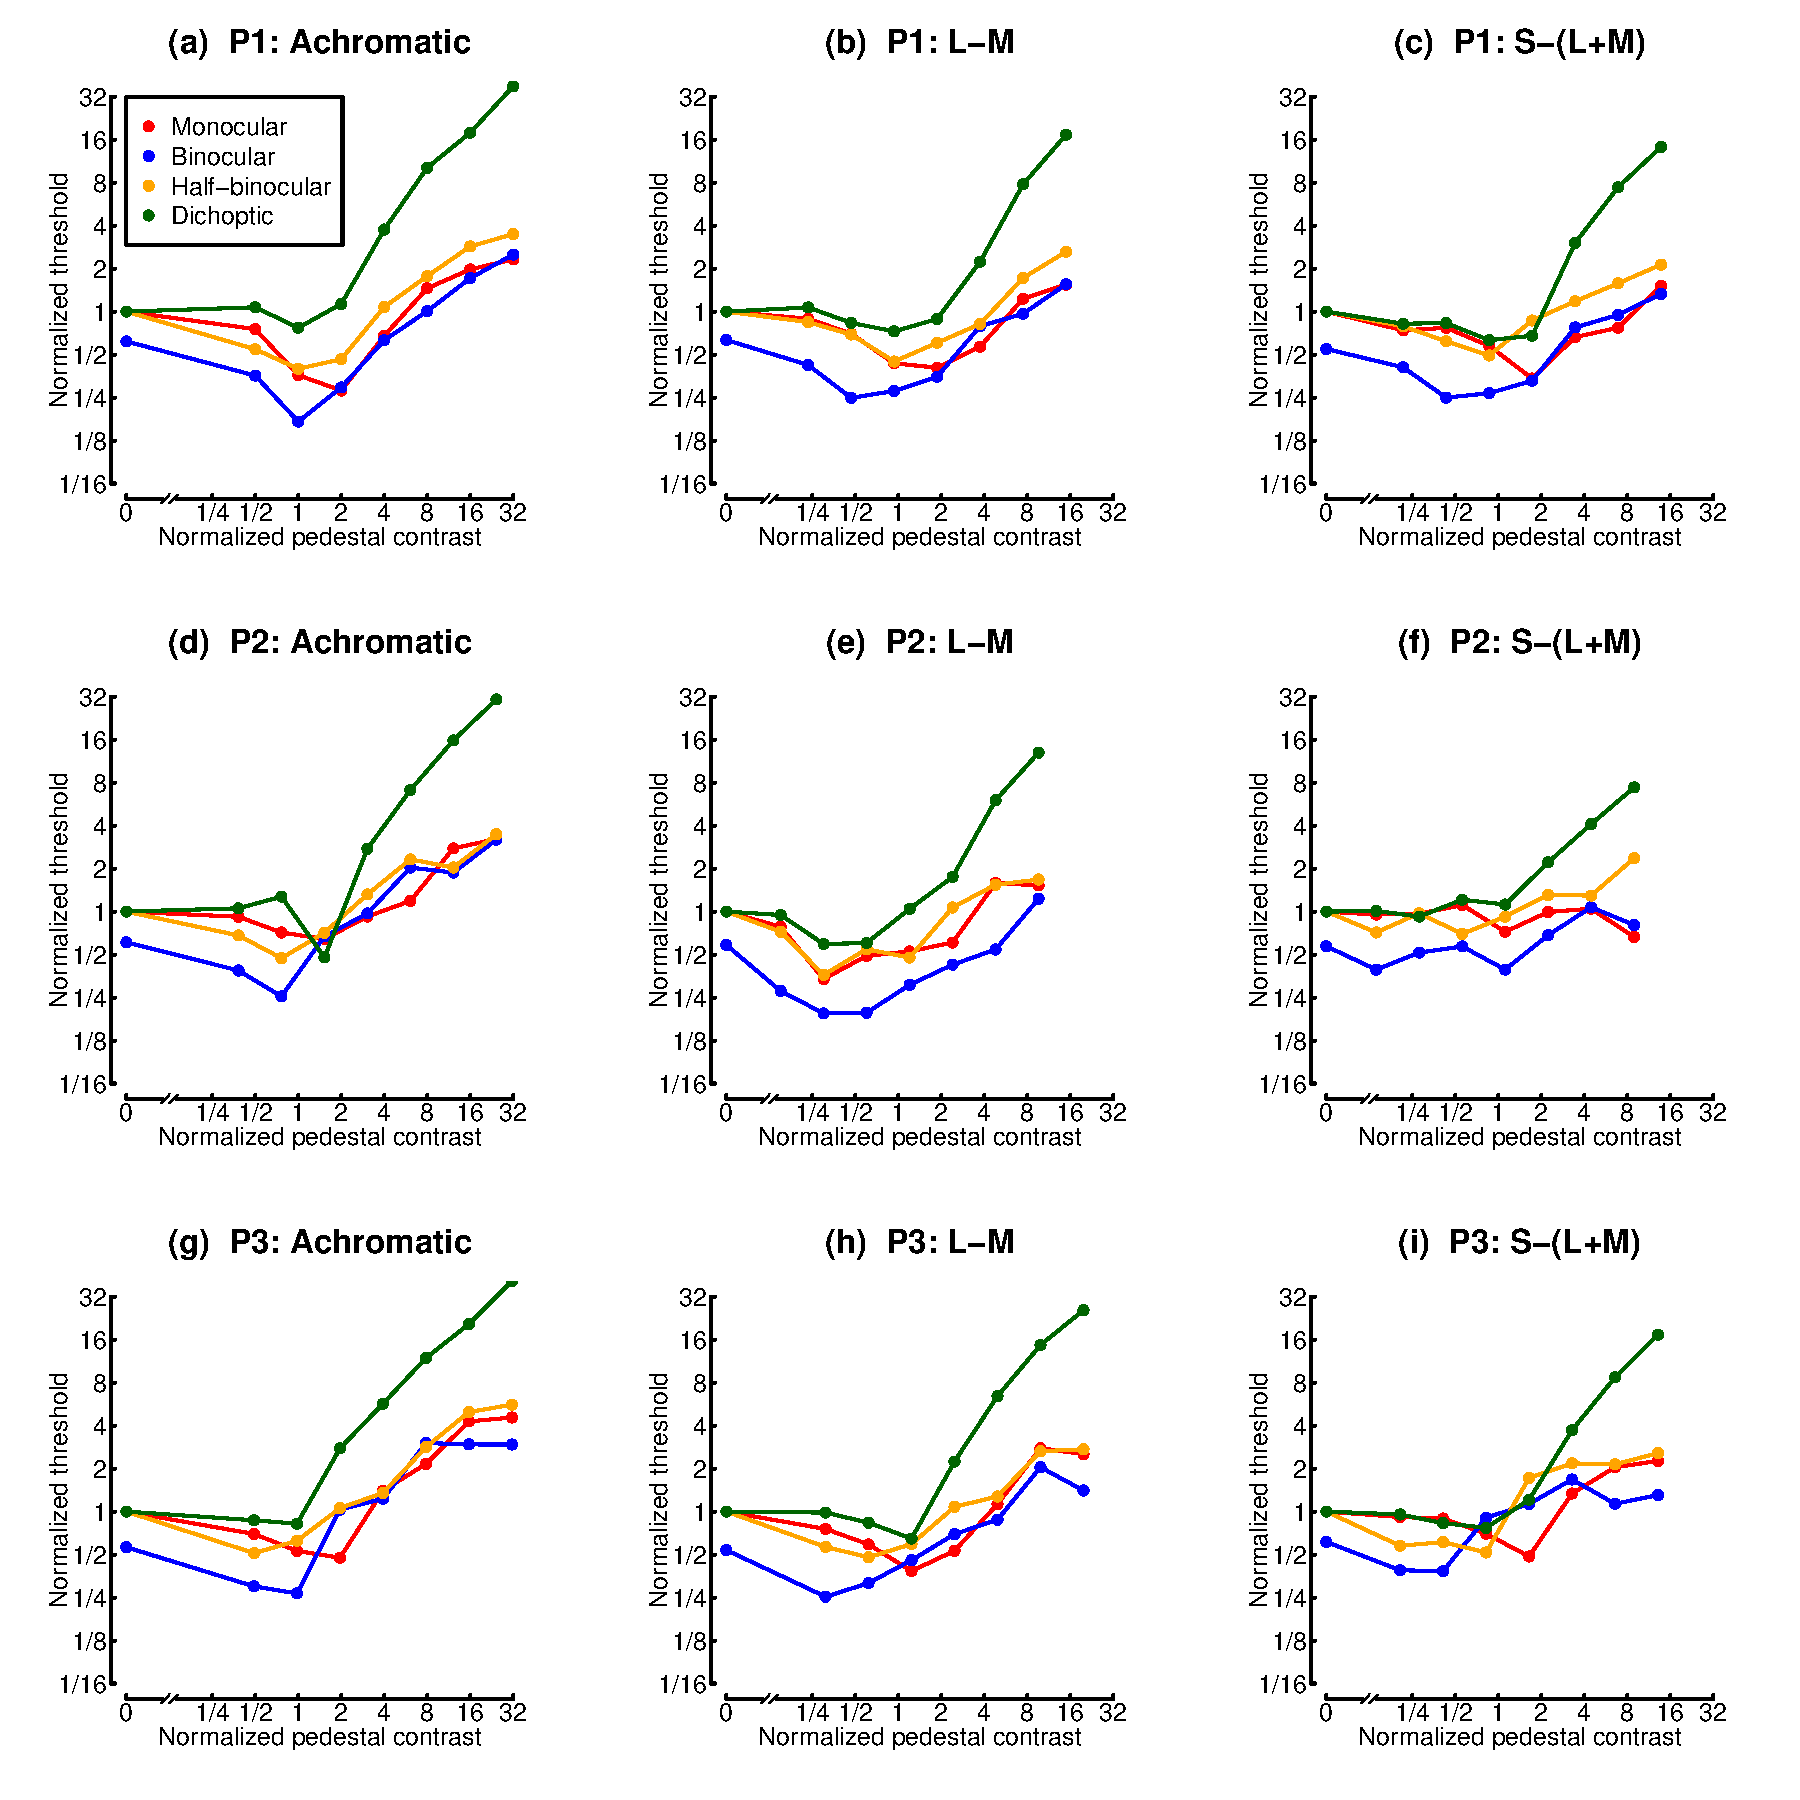
\includegraphics{Figures/individualdippers} 

}

\caption{Individual participant data from Experiment 1.}\label{fig:individualdips}
\end{figure}

\begin{figure}

{\centering 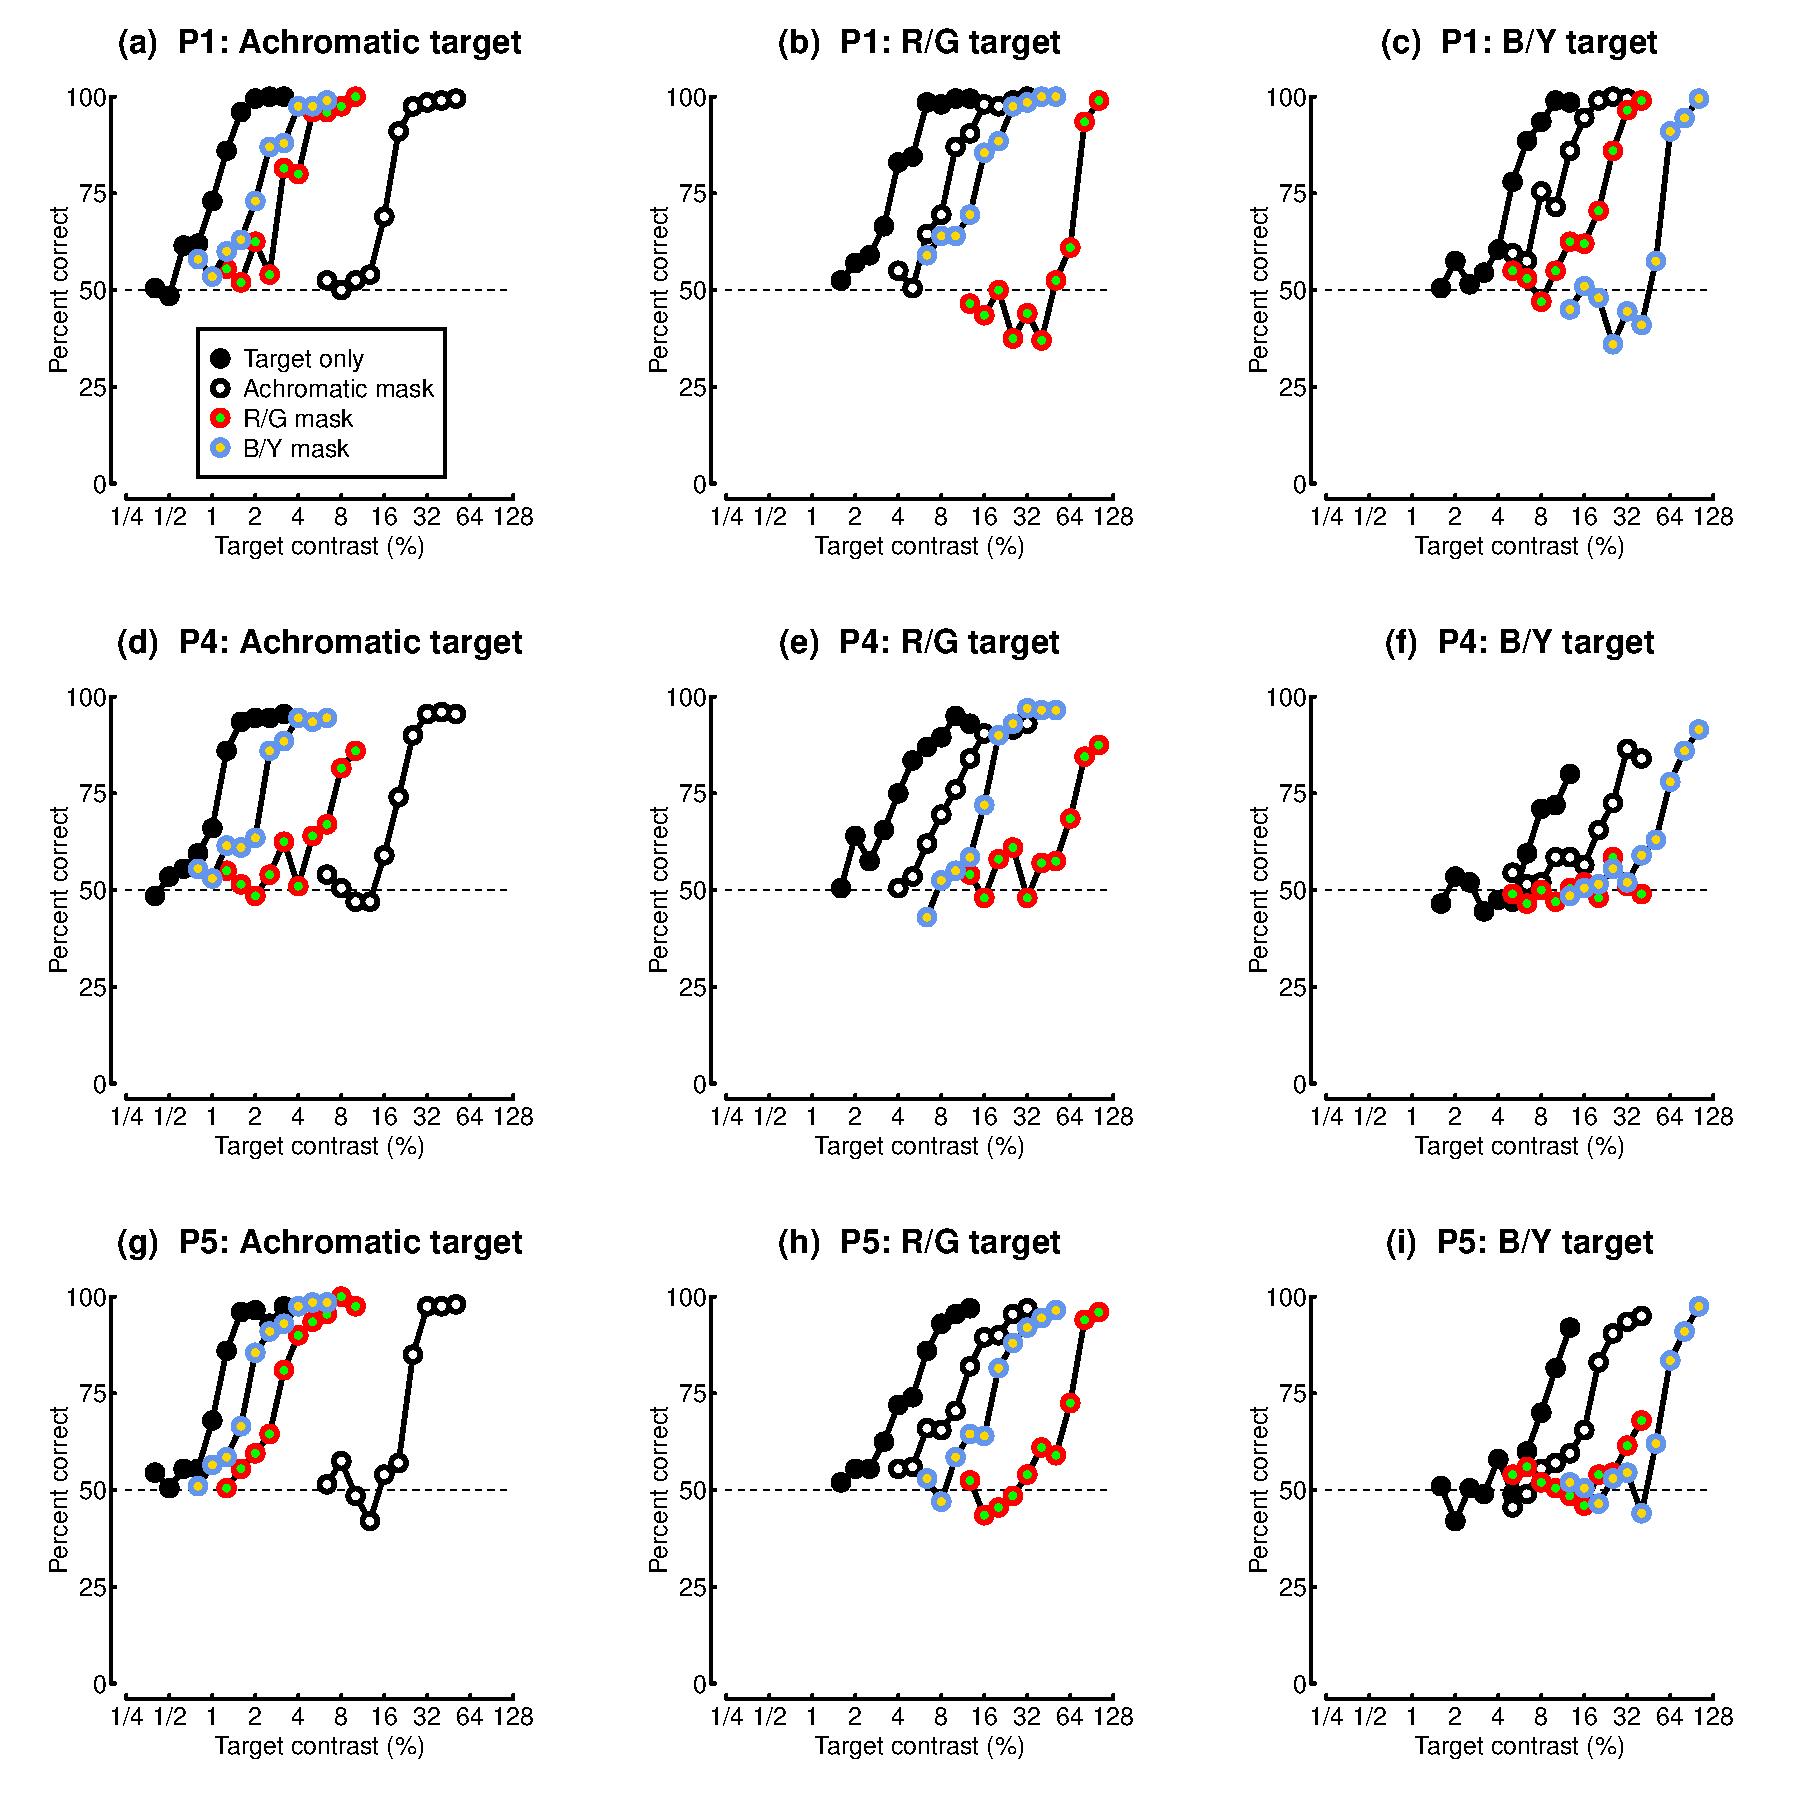
\includegraphics{Figures/individualMCS} 

}

\caption{Individual participant data from Experiment 2.}\label{fig:individualMCS}
\end{figure}

\end{document}
